\documentclass{beamer}
\setbeamerfont{headline}{size=\footnotesize}

\mode<presentation>{
\usetheme{Montpellier}
\setbeamercovered{transparent}
\usecolortheme{lsc}
}

\mode<handout>{
  % tema simples para ser impresso
  \usepackage[bar]{beamerthemetree}
   % Colocando um fundo cinza quando for gerar transparências para serem impressas
  % mais de uma transparência por página
  \beamertemplatesolidbackgroundcolor{black!5}
}

\usepackage{fancyvrb}
\usepackage{pdfpages} % Pacote para incluir PDFs

\usepackage{amsmath,amssymb}
\usepackage[brazil]{varioref}
\usepackage[english,brazil]{babel}
\usepackage[utf8]{inputenc}
\usepackage{fontawesome}
\usepackage{ccicons}

\usepackage{makecell} % Adicione isso no preâmbulo do documento

%\usepackage[latin1]{inputenc}
\usepackage{graphicx}
\usepackage{listings}
\usepackage{url}
\usepackage{colortbl}
\usepackage{caption}
\usepackage{tikz}
\usepackage{transparent}
\usepackage{multirow}
\usepackage{graphicx}
\usepackage{listings}
\usepackage{exercise,chngcntr}

\usepackage{listings}
\usepackage{xcolor}
\usepackage{tikz}
\usetikzlibrary{shapes, arrows.meta, positioning}


% Definição de cores para o código Python
\definecolor{codegreen}{rgb}{0,0.6,0}
\definecolor{codegray}{rgb}{0.5,0.5,0.5}
\definecolor{codepurple}{rgb}{0.58,0,0.82}
\definecolor{backcolour}{rgb}{0.95,0.95,0.92}
% Configuração do estilo do código Python
\lstdefinestyle{mystyle}{
    xleftmargin=0pt,           % Aumenta a margem esquerda
    xrightmargin=10pt,          % Aumenta a margem direita
    frame=single,               % Adiciona um quadro ao redor do código
    framesep=10pt,              % Espaço entre o quadro e o código
    % Outras configurações do lstlisting...
    backgroundcolor=\color{backcolour},
    commentstyle=\color{codegreen},
    keywordstyle=\color{magenta},
    numberstyle=\tiny\color{codegray},
    stringstyle=\color{codepurple},
    basicstyle=\footnotesize\ttfamily,
    breakatwhitespace=false,
    breaklines=true,
    captionpos=b,
    keepspaces=true,
    %numbers=left,
    numbersep=5pt,
    showspaces=false,
    showstringspaces=false,
    showtabs=false,
    tabsize=2,
    basicstyle=\ttfamily, % Usa uma fonte de largura fixa para o código
    upquote=true,         % Tenta usar aspas retas se a fonte suportar,
    breakatwhitespace=false, % Quebra linhas em espaços em branco quando possível
}

\lstset{style=mystyle}


\beamertemplatetransparentcovereddynamic
\addtobeamertemplate{title page}{\centering{ 
\includegraphics[width=1.25cm]{figs/logo.png}}}{}
\title[]{Introdução ao LangChain}
\author[Elton Sarmanho]{ 
Professor: Elton Sarmanho\inst{1} 
\newline
E-mail: \href{mailto:eltonss@ufpa.br}{eltonss@ufpa.br}\newline
\href{https://github.com/eltonsarmanho}{\faGithub} \href{https://www.linkedin.com/in/elton-sarmanho-836553185/}{\faLinkedinSquare}\\
\ccbyncsa
}   
  \institute[UFPA]{
   \inst{1}%
     Faculdade de Sistemas de Informação - UFPA/CUNTINS
     }     
 
% Se comentar a linha abaixo, irá aparecer a data quando foi compilada a apresentação  
\date{\today}
\pgfdeclareimage[height= 1.25 cm]{inf}{figs/logo.png}
% pode-se colocar o LOGO assim
\logo{{\transparent{0.35}\pgfuseimage{inf}}}

% \AtBeginSection[]{
%   \begin{frame}<beamer>
%     \frametitle{Roteiro}
%     \tableofcontents[currentsection,currentsubsection]
%   \end{frame}  
% }

\setbeamertemplate{navigation symbols}{\insertframenavigationsymbol \insertsectionnavigationsymbol \insertbackfindforwardnavigationsymbol} 


\expandafter\def\expandafter\insertshorttitle\expandafter{%
  \insertshorttitle\hfill%
  \insertframenumber\,/\,\inserttotalframenumber}
  \renewcounter{Exercise}[section]
  \newcounter{Example}



\begin{document}

\setbeamertemplate{logo}{}
\begin{frame}
\titlepage
\end{frame}
%Começar mostrar Logo apos slide de titulo
\logo{{\transparent{0.35}\pgfuseimage{inf}}}

\begin{frame}
\frametitle{Roteiro}
\tableofcontents[sections={1-3}]
\end{frame}
\begin{frame}
\frametitle{Roteiro}
\tableofcontents[sections={4-6}]
\end{frame}

\begin{frame}
\frametitle{Roteiro}
\tableofcontents[sections={7-8}]
\end{frame}
\begin{frame}{Licença}
    Este trabalho está licenciado sob a licença Creative Commons:

    \bigskip
    \ccbyncsa
\end{frame}
%Declaração das Imagens da Apresentação

%%%%%%%%%%%%%%%%%%%%%%%%%%%%%%%%%%%%%%%%
\section{Planejamento}

\begin{frame}
Nesta aula:

\begin{itemize}
     \item Compreender o que são Modelos de Linguagem (LLMs).
    \item Entender o conceito de Cadeias (Chains) no LangChain.
    \item Introduzir a base matemática e computacional por trás dos LLMs.
    \item Explorar exemplos práticos de uso de LLMs e Chains.
 \item Códigos do Professor estão no github
\end{itemize}


\end{frame}
\section{Fundamentação}
\subsection{Conceitos Fundamentais}
\begin{frame}
\centering
\Huge
\textbf{Conceitos\\Fundamentais}
\end{frame}
\begin{frame}{O que são Modelos de Linguagem (LLMs)?}
\begin{itemize}
    \item Modelos de linguagem são sistemas de inteligência artificial treinados para gerar e entender texto.
    \item Baseados em arquiteturas de redes neurais, como Transformers.
    \item Exemplos: GPT-3, GPT-4, BERT, etc.
\end{itemize}
   \centering

\begin{tikzpicture}
    \node[draw, fill=blue!20, minimum width=3cm, minimum height=1cm] (llm) at (0,0) {LLM};
    \node[draw, fill=green!20, minimum width=3cm, minimum height=1cm] (input) at (-3, 1.5) {Entrada};
    \node[draw, fill=red!20, minimum width=3cm, minimum height=1cm] (output) at (3, 1.5) {Saída};

    \draw[->] (input) -- (llm);
    \draw[->] (llm) -- (output);
\end{tikzpicture}
\end{frame}



% Slide 3 - Representação Matemática de um LLM
\begin{frame}{Modelos de Linguagem e Representação Matemática}
    Um LLM pode ser visto como uma função:
    \begin{equation}
        f(x) = P(y | x; \theta)
    \end{equation}
    Onde:
    \begin{itemize}
        \item $x$ é a entrada textual;
        \item $y$ é a saída gerada;
        \item $\theta$ são os parâmetros do modelo.
    \end{itemize}
    \textbf{O LangChain encapsula essa função para criar fluxos mais complexos de IA.}
\end{frame}

\begin{frame}{Por que LangChain?}
    \begin{itemize}
        \item Grandes Modelos de Linguagem (LLMs) revolucionaram o processamento de texto.
        \item LangChain permite criar aplicações avançadas de IA baseadas em LLMs.
        \item Foca em pipelines modulares para fácil integração com dados externos.
    \end{itemize}
\end{frame}


% Slide 2 - Arquitetura do LangChain
\begin{frame}{Arquitetura do LangChain}
    \begin{itemize}
        \item \textbf{Modelos}: OpenAI, Hugging Face, Sabiá 2.
        \item \textbf{Cadeias (Chains)}: Conectam múltiplas operações de IA.
        \item \textbf{Agentes (Agents)}: Tomam decisões com base em entradas dinâmicas.
        \item \textbf{Memória}: Armazena contexto de conversas anteriores.
        \item \textbf{Bases de Dados Vetoriais}: FAISS, Pinecone, ChromaDB.
    \end{itemize}
\end{frame}

\begin{frame}{O que são Cadeias (Chains) no LangChain?}
\begin{itemize}
    \item Cadeias são sequências de chamadas a modelos ou outras funções que são executadas em uma ordem específica.
    \item Exemplo: Uma cadeia pode envolver a chamada a um modelo de linguagem, seguida por uma chamada a uma API externa, e então a geração de uma resposta final.
\end{itemize}
   \centering

\begin{tikzpicture}
    \node[draw, fill=blue!20, minimum width=2cm, minimum height=1cm] (llm) at (0,0) {LLM};
    \node[draw, fill=green!20, minimum width=2cm, minimum height=1cm] (api) at (3,0) {API};
    \node[draw, fill=red!20, minimum width=2cm, minimum height=1cm] (output) at (6,0) {Saída};

    \draw[->] (llm) -- (api);
    \draw[->] (api) -- (output);
\end{tikzpicture}
\end{frame}

% Slide 4 - Diagrama de Fluxo com TikZ
\begin{frame}{Fluxo de uma Cadeia no LangChain}
    \begin{center}
        \begin{tikzpicture}[node distance=1.5cm, auto]
            \node (input) [rectangle, draw] {Entrada do Usuário};
            \node (model) [rectangle, draw, below of=input] {LLM [\textbf{CHAIN 1}]};
            \node (process) [rectangle, draw, below of=model] {Pós-processamento [\textbf{CHAIN 2}]};
            \node (output) [rectangle, draw, below of=process] {Saída para o Usuário};

            \draw [->] (input) -- (model);
            \draw [->] (model) -- (process);
            \draw [->] (process) -- (output);
        \end{tikzpicture}
    \end{center}
\end{frame}

% Slide 5 - Exemplo Prático
\begin{frame}[fragile]{Exemplo de Código em Python}
    \begin{verbatim}
    from langchain.llms import OpenAI
    llm = OpenAI(model_name="gpt-4")
    resposta = llm.predict("o que e buraco negro")
    print(resposta)
    \end{verbatim}
\end{frame}



\begin{frame}{Exemplo Prático de uma Cadeia}
\begin{itemize}
    \item Considere uma cadeia que:
    \begin{enumerate}
        \item Recebe uma pergunta do usuário.
        \item Chama um modelo de linguagem para gerar uma resposta preliminar.
        \item Chama uma API de tradução para traduzir a resposta para outro idioma.
        \item Retorna a resposta traduzida ao usuário.
    \end{enumerate}
\end{itemize}

\begin{tikzpicture}
    \node[draw, fill=blue!20, minimum width=2cm, minimum height=1cm] (input) at (0,0) {Pergunta};
    \node[draw, fill=green!20, minimum width=2cm, minimum height=1cm] (llm) at (3,0) {LLM};
    \node[draw, fill=red!20, minimum width=2cm, minimum height=1cm] (api) at (6,0) {API Trad.};
    \node[draw, fill=yellow!20, minimum width=2cm, minimum height=1cm] (output) at (9,0) {Resposta};

    \draw[->] (input) -- (llm);
    \draw[->] (llm) -- (api);
    \draw[->] (api) -- (output);
\end{tikzpicture}
\end{frame}

\section{Trabalhando com Modelos de Linguagem}
\begin{frame}
\centering
\Huge
\textbf{Modelos\\de Linguagem}
\end{frame}
% Módulo 2 - Trabalhando com Modelos de Linguagem
\begin{frame}{Modelos de Linguagem}
    \begin{itemize}
        \item Como LangChain se conecta a diferentes modelos de LLMs.
        \item Importância do ajuste fino dos prompts.
        \item Estratégias de otimização de desempenho.
    \end{itemize}
\end{frame}

% Slide - Seleção de Modelos
\begin{frame}{Escolha do Modelo Adequado}
    \begin{itemize}
        \item Modelos open-source vs. modelos proprietários.
        \item Custo-benefício na utilização de LLMs.
        \item Comparação de latência e acurácia.
    \end{itemize}
\end{frame}

% Slide - Representação de Embeddings
\begin{frame}{Embeddings e Representação Vetorial}
    \textbf{Definição}: Representação numérica de palavras/sentenças para cálculos matemáticos.
    \begin{equation}
        E(w) = \mathbf{v} \in \mathbb{R}^d
    \end{equation}
    Onde $d$ é a dimensão do espaço vetorial e $\mathbf{v}$ é o vetor associado à palavra $w$.
\end{frame}
\begin{frame}{Espaço Vetorial de Embeddings}
    \begin{center}
        \begin{tikzpicture}
            \draw[->] (-1,0) -- (3,0) node[right] {$x_1$};
            \draw[->] (0,-1) -- (0,3) node[above] {$x_2$};
            \node[draw, circle, fill=blue!20] at (1,2) {palavra1};
            \node[draw, circle, fill=red!20] at (2,1) {palavra2};
            \node[draw, circle, fill=green!20] at (1.5,1.5) {palavra3};
        \end{tikzpicture}
    \end{center}
\end{frame}
\section{Agentes e Memória no LangChain}
\begin{frame}
\centering
\Huge
\textbf{Agentes\\Memória no LangChain}
\end{frame}
\begin{frame}{Objetivos}
\begin{itemize}
    \item Compreender o conceito de Agentes no LangChain.
    \item Entender como a Memória é usada para manter o contexto.
    \item Explorar a base matemática e computacional por trás dos Agentes.
    \item Ver exemplos práticos de Agentes e Memória em ação.
\end{itemize}
\end{frame}

\begin{frame}{O que são Agentes no LangChain?}
\begin{itemize}
    \item Agentes são componentes que tomam decisões sobre quais ações executar com base em entradas e contextos específicos.
    \item Eles podem decidir qual modelo chamar, qual API usar, ou até mesmo qual cadeia de ações executar.
    \item Exemplos: \texttt{ZeroShotAgent}, \texttt{ReActAgent}.
\end{itemize}
   \centering

\begin{tikzpicture}
    \node[draw, fill=blue!20, minimum width=3cm, minimum height=1cm] (agent) at (0,0) {Agente};
    \node[draw, fill=green!20, minimum width=2cm, minimum height=1cm] (input) at (-3, 1.5) {Entrada};
    \node[draw, fill=red!20, minimum width=2cm, minimum height=1cm] (action) at (3, 1.5) {Ação};

    \draw[->] (input) -- (agent);
    \draw[->] (agent) -- (action);
\end{tikzpicture}
\end{frame}

\begin{frame}{Base Computacional dos Agentes}
\begin{itemize}
    \item Agentes usam técnicas de \textbf{planejamento} e \textbf{tomada de decisão} para escolher a melhor ação.
    \item Podem ser modelados como um problema de \textbf{otimização}:
    \[
    \text{Ação}^* = \arg\max_{a \in A} \; P(a \mid \text{Entrada}, \text{Contexto})
    \]
    onde:
    \begin{itemize}
        \item \( A \): Conjunto de ações possíveis.
        \item \( P \): Função de probabilidade que avalia a adequação da ação.
    \end{itemize}
\end{itemize}
   \centering

\begin{tikzpicture}
    \node[draw, fill=blue!20, minimum width=2cm, minimum height=1cm] (agent) at (0,0) {Agente};
    \node[draw, fill=green!20, minimum width=1.5cm, minimum height=1cm] (input) at (-2, 1.5) {Entrada};
    \node[draw, fill=yellow!20, minimum width=1.5cm, minimum height=1cm] (context) at (0, 1.5) {Contexto};
    \node[draw, fill=red!20, minimum width=1.5cm, minimum height=1cm] (action) at (2, 1.5) {Ação};

    \draw[->] (input) -- (agent);
    \draw[->] (context) -- (agent);
    \draw[->] (agent) -- (action);
\end{tikzpicture}
\end{frame}

\begin{frame}{O que é Memória no LangChain?}
\begin{itemize}
    \item Memória é a capacidade de armazenar e recuperar informações entre diferentes interações ou chamadas.
    \item Mantém o contexto de uma conversa ou de um fluxo de trabalho.
    \item Exemplos: \texttt{ConversationBufferMemory}, \texttt{ConversationSummaryMemory}.
\end{itemize}
   \centering

\begin{tikzpicture}
    \node[draw, fill=blue!20, minimum width=3cm, minimum height=1cm] (memory) at (0,0) {Memória};
    \node[draw, fill=green!20, minimum width=2cm, minimum height=1cm] (input) at (-3, 1.5) {Entrada};
    \node[draw, fill=red!20, minimum width=2cm, minimum height=1cm] (output) at (3, 1.5) {Saída};

    \draw[->] (input) -- (memory);
    \draw[->] (memory) -- (output);
    \draw[->] (output) to[out=270,in=270] (memory);
\end{tikzpicture}
\end{frame}

\begin{frame}{Estrutura da Memória}
\footnotesize
\begin{itemize}
    \item A memória pode ser modelada como um \textbf{estado} \( S \) que evolui ao longo do tempo:
    \[
    S_{t+1} = f(S_t, \text{Entrada}_t)
    \]
    onde:
    \begin{itemize}
        \item \( S_t \): Estado atual da memória.
        \item \( \text{Entrada}_t \): Nova entrada no tempo \( t \).
        \item \( f \): Função de atualização do estado.
    \end{itemize}
    \item A saída é gerada com base no estado atual:
    \[
    \text{Saída}_t = g(S_t)
    \]
\end{itemize}
   \centering

\begin{tikzpicture}
    \node[draw, fill=blue!20, minimum width=2cm, minimum height=1cm] (memory) at (0,0) {Memória};
    \node[draw, fill=green!20, minimum width=1.5cm, minimum height=1cm] (input) at (-2, 1.5) {Entrada};
    \node[draw, fill=red!20, minimum width=1.5cm, minimum height=1cm] (output) at (2, 1.5) {Saída};

    \draw[->] (input) -- (memory);
    \draw[->] (memory) -- (output);
    \draw[->] (output) to[out=270,in=270] (memory);
\end{tikzpicture}
\end{frame}

\begin{frame}{Exemplo Prático de Agente com Memória}
\begin{itemize}
    \item Considere um agente que:
    \begin{enumerate}
        \item Recebe uma pergunta do usuário.
        \item Usa a memória para manter o contexto da conversa.
        \item Decide qual ação tomar (ex.: chamar um modelo de linguagem ou uma API).
        \item Retorna a resposta ao usuário e atualiza a memória.
    \end{enumerate}
\end{itemize}
   \centering

\begin{tikzpicture}
    \node[draw, fill=blue!20, minimum width=2cm, minimum height=1cm] (agent) at (0,0) {Agente};
    \node[draw, fill=green!20, minimum width=1.5cm, minimum height=1cm] (input) at (-3, 1.5) {Pergunta};
    \node[draw, fill=yellow!20, minimum width=1.5cm, minimum height=1cm] (memory) at (0, 1.5) {Memória};
    \node[draw, fill=red!20, minimum width=1.5cm, minimum height=1cm] (output) at (3, 1.5) {Resposta};

    \draw[->] (input) -- (agent);
    \draw[->] (memory) -- (agent);
    \draw[->] (agent) -- (output);
    \draw[->] (output) to[out=270,in=270] (memory);
\end{tikzpicture}
\end{frame}



\section{Prompts e Indexação no LangChain}
\begin{frame}
\centering
\Huge
\textbf{Prompts\\Indexação no LangChain}
\end{frame}

\begin{frame}{Objetivos do Módulo}
\begin{itemize}
    \item Compreender o conceito de Prompts no LangChain.
    \item Entender como a Indexação e Recuperação de informações funcionam.
    \item Explorar a base matemática e computacional por trás dos Prompts.
    \item Ver exemplos práticos de Prompts e Indexação em ação.
\end{itemize}
\end{frame}

\begin{frame}{O que são Prompts no LangChain?}
\begin{itemize}
    \item Prompts são textos ou instruções que são fornecidos ao modelo de linguagem para guiar sua geração de texto.
    \item Podem ser estáticos ou dinâmicos, dependendo do contexto.
    \item Exemplos: \texttt{PromptTemplate}, \texttt{FewShotPromptTemplate}.
\end{itemize}
   \centering

\begin{tikzpicture}
    \node[draw, fill=blue!20, minimum width=3cm, minimum height=1cm] (prompt) at (0,0) {Prompt};
    \node[draw, fill=green!20, minimum width=2cm, minimum height=1cm] (input) at (-3, 1.5) {Entrada};
    \node[draw, fill=red!20, minimum width=2cm, minimum height=1cm] (output) at (3, 1.5) {Saída};

    \draw[->] (input) -- (prompt);
    \draw[->] (prompt) -- (output);
\end{tikzpicture}
\end{frame}

\begin{frame}{Base dos Prompts}
\begin{itemize}
    \item Prompts podem ser vistos como uma função \( f \) que mapeia uma entrada \( x \) para uma saída \( y \):
    \[
    y = f(x, \theta)
    \]
    onde:
    \begin{itemize}
        \item \( x \): Entrada do usuário.
        \item \( \theta \): Parâmetros do prompt (ex.: instruções, exemplos).
        \item \( y \): Saída gerada pelo modelo.
    \end{itemize}
    \item Em prompts dinâmicos, \( \theta \) pode variar com base no contexto.
\end{itemize}
   \centering

\begin{tikzpicture}
    \node[draw, fill=blue!20, minimum width=2cm, minimum height=1cm] (prompt) at (0,0) {Prompt};
    \node[draw, fill=green!20, minimum width=1.5cm, minimum height=1cm] (input) at (-2, 1.5) {Entrada};
    \node[draw, fill=yellow!20, minimum width=1.5cm, minimum height=1cm] (params) at (0, 1.5) {Parâmetros};
    \node[draw, fill=red!20, minimum width=1.5cm, minimum height=1cm] (output) at (2, 1.5) {Saída};

    \draw[->] (input) -- (prompt);
    \draw[->] (params) -- (prompt);
    \draw[->] (prompt) -- (output);
\end{tikzpicture}
\end{frame}

\begin{frame}{Indexação e Recuperação no LangChain}
\begin{itemize}
    \item Indexação é o processo de organizar documentos ou dados para facilitar a recuperação.
    \item Recuperação é o processo de buscar informações relevantes com base em uma consulta.
    \item Exemplos: \texttt{VectorStore}, \texttt{Retriever}.
\end{itemize}
   \centering

\begin{tikzpicture}
    \node[draw, fill=blue!20, minimum width=3cm, minimum height=1cm] (index) at (0,0) {Indexação};
    \node[draw, fill=green!20, minimum width=2cm, minimum height=1cm] (docs) at (-3, 1.5) {Documentos};
    \node[draw, fill=red!20, minimum width=2cm, minimum height=1cm] (query) at (3, 1.5) {Consulta};

    \draw[->] (docs) -- (index);
    \draw[->] (query) -- (index);
    \draw[->] (index) -- (0, -1.5) node[below] {Resultados};
\end{tikzpicture}
\end{frame}

\begin{frame}{Estrutura da Indexação e Recuperação}
\footnotesize
\begin{itemize}
    \item A indexação pode ser modelada como um problema de similaridade:
    \[
    \text{Similaridade}(q, d) = \frac{q \cdot d}{\|q\| \|d\|}
    \]
    onde:
    \begin{itemize}
        \item \( q \): Vetor de consulta.
        \item \( d \): Vetor de documento.
    \end{itemize}
    \item A recuperação busca maximizar a similaridade entre a consulta e os documentos.
\end{itemize}
   \centering

\begin{tikzpicture}
    \node[draw, fill=blue!20, minimum width=2cm, minimum height=1cm] (index) at (0,0) {Indexação};
    \node[draw, fill=green!20, minimum width=1.5cm, minimum height=1cm] (docs) at (-2, 1.5) {Documentos};
    \node[draw, fill=red!20, minimum width=1.5cm, minimum height=1cm] (query) at (2, 1.5) {Consulta};

    \draw[->] (docs) -- (index);
    \draw[->] (query) -- (index);
    \draw[->] (index) -- (0, -0.75) node[below] {Resultados};
\end{tikzpicture}
\end{frame}

\begin{frame}{Exemplo Prático de Prompts e Indexação}
\begin{itemize}
    \item Considere um sistema que:
    \begin{enumerate}
        \item Recebe uma pergunta do usuário.
        \item Usa um prompt para gerar uma consulta.
        \item Recupera documentos relevantes de um índice.
        \item Gera uma resposta com base nos documentos recuperados.
    \end{enumerate}
\end{itemize}
   \centering

\begin{tikzpicture}
    \node[draw, fill=blue!20, minimum width=2cm, minimum height=1cm] (prompt) at (0,0) {Prompt};
    \node[draw, fill=green!20, minimum width=1.5cm, minimum height=1cm] (input) at (-3, 1.5) {Pergunta};
    \node[draw, fill=yellow!20, minimum width=1.5cm, minimum height=1cm] (index) at (0, 1.5) {Indexação};
    \node[draw, fill=red!20, minimum width=1.5cm, minimum height=1cm] (output) at (3, 1.5) {Resposta};

    \draw[->] (input) -- (prompt);
    \draw[->] (prompt) -- (index);
    \draw[->] (index) -- (output);
\end{tikzpicture}
\end{frame}

\section{Python com LangChain}
\begin{frame}
\centering
 \begin{figure}[h]
         \centering
         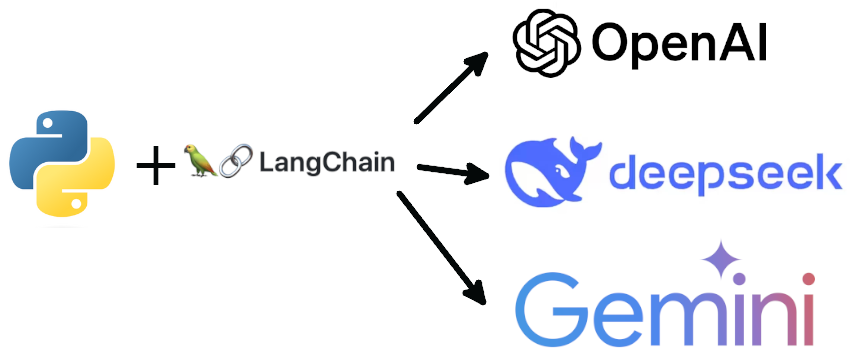
\includegraphics[width=0.9\textwidth]{figs/python.png}
    \end{figure}
\end{frame}

\begin{frame}
\centering
 \begin{figure}[h]
         \centering
         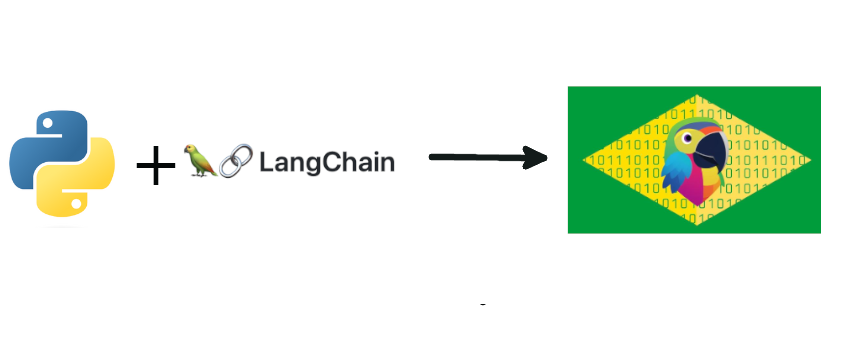
\includegraphics[width=0.9\textwidth]{figs/python2.png}
    \end{figure}
\end{frame}

\begin{frame}{Objetivos}
\begin{itemize}
    \item Explorar a integração de Python com ferramentas avançadas como OpenAI, LangChain, DeepSeek e Gemini.
    \item Fornecer exemplos práticos de uso de Python.
\end{itemize}

\end{frame}

\begin{frame}{O que é Python?}
\begin{itemize}
    \item Python é uma linguagem de programação de alto nível, interpretada e de propósito geral.
    \item Conhecida por sua sintaxe simples e legibilidade.
    \item Amplamente utilizada em áreas como desenvolvimento web, ciência de dados, automação e inteligência artificial.
\end{itemize}
   \centering
\begin{tikzpicture}
    \node[draw, fill=blue!20, minimum width=3cm, minimum height=1cm] (python) at (0,0) {Python};
    \node[draw, fill=green!20, minimum width=2cm, minimum height=1cm] (web) at (-3, 1.5) {Desenvolvimento Web};
    \node[draw, fill=red!20, minimum width=2cm, minimum height=1cm] (ai) at (3, 1.5) {Inteligência Artificial};

    \draw[->] (python) -- (web);
    \draw[->] (python) -- (ai);
\end{tikzpicture}
\end{frame}

\begin{frame}{Integração com OpenAI}
\begin{itemize}
    \item OpenAI fornece modelos de linguagem avançados como GPT-3 e GPT-4.
    \item Python pode ser usado para integrar esses modelos em aplicações.
    \item Exemplo: Uso da API da OpenAI para gerar texto.
\end{itemize}
   \centering
\begin{tikzpicture}
    \node[draw, fill=blue!20, minimum width=3cm, minimum height=1cm] (python) at (0,0) {Python};
    \node[draw, fill=green!20, minimum width=2cm, minimum height=1cm] (openai) at (3,0) {OpenAI};

    \draw[->] (python) -- (openai);
\end{tikzpicture}
\end{frame}

\begin{frame}{Integração com LangChain}
\begin{itemize}
    \item LangChain é uma estrutura para construir aplicações com modelos de linguagem.
    \item Python é a linguagem principal para trabalhar com LangChain.
    \item Exemplo: Criação de cadeias de processamento de linguagem natural.
\end{itemize}
   \centering
\begin{tikzpicture}
    \node[draw, fill=blue!20, minimum width=3cm, minimum height=1cm] (python) at (0,0) {Python};
    \node[draw, fill=green!20, minimum width=2cm, minimum height=1cm] (langchain) at (3,0) {LangChain};

    \draw[->] (python) -- (langchain);
\end{tikzpicture}
\end{frame}

\begin{frame}{Integração com DeepSeek}
\begin{itemize}
    \item DeepSeek é uma plataforma para análise de dados e machine learning.
    \item Python pode ser usado para integrar DeepSeek em pipelines de dados.
    \item Exemplo: Análise de grandes volumes de dados com DeepSeek.
\end{itemize}
   \centering
\begin{tikzpicture}
    \node[draw, fill=blue!20, minimum width=3cm, minimum height=1cm] (python) at (0,0) {Python};
    \node[draw, fill=green!20, minimum width=2cm, minimum height=1cm] (deepseek) at (3,0) {DeepSeek};

    \draw[->] (python) -- (deepseek);
\end{tikzpicture}
\end{frame}

\begin{frame}{Integração com Gemini}
\begin{itemize}
    \item Gemini é uma plataforma para desenvolvimento de aplicações blockchain.
    \item Python pode ser usado para interagir com a blockchain via Gemini.
    \item Exemplo: Criação de smart contracts e transações.
\end{itemize}
   \centering
\begin{tikzpicture}
    \node[draw, fill=blue!20, minimum width=3cm, minimum height=1cm] (python) at (0,0) {Python};
    \node[draw, fill=green!20, minimum width=2cm, minimum height=1cm] (gemini) at (3,0) {Gemini};

    \draw[->] (python) -- (gemini);
\end{tikzpicture}
\end{frame}

\begin{frame}{Exemplo Prático de Uso de Python}
\begin{itemize}
    \item Considere um projeto que:
    \begin{enumerate}
        \item Coleta dados de uma API.
        \item Processa os dados usando Python.
        \item Integra com OpenAI para análise de texto.
        \item Armazena os resultados em um banco de dados.
    \end{enumerate}
\end{itemize}
   \centering
\begin{tikzpicture}
    \node[draw, fill=blue!20, minimum width=2cm, minimum height=1cm] (python) at (0,0) {Python};
    \node[draw, fill=green!20, minimum width=1.5cm, minimum height=1cm] (api) at (-2, 1.5) {API};
    \node[draw, fill=yellow!20, minimum width=1.5cm, minimum height=1cm] (openai) at (0, 1.5) {OpenAI};
    \node[draw, fill=red!20, minimum width=1.5cm, minimum height=1cm] (db) at (3, 1.5) {Banco de Dados};

    \draw[->] (api) -- (python);
    \draw[->] (python) -- (openai);
    \draw[->] (openai) -- (db);
\end{tikzpicture}
\end{frame}

\section{Retrieval Augmented Generation (RAG)}
\begin{frame}
\centering
\Huge
\textbf{RAG}
\end{frame}

\begin{frame}{Objetivos do Módulo}
\begin{itemize}
    \item Compreender o conceito de Retrieval Augmented Generation (RAG).
        \item Aprender a implementar RAG usando LangChain.
    \item Ver exemplos práticos de RAG em ação.
\end{itemize}
\end{frame}

\begin{frame}{O que é Retrieval Augmented Generation (RAG)?}
\footnotesize
\begin{itemize}
    \item RAG combina recuperação de informações com geração de texto.
    \item Usa um sistema de recuperação para buscar documentos (partes) relevantes.
    \item Gera respostas com base nos documentos recuperados.
\end{itemize}
\centering
\begin{tikzpicture}
    \node[draw, fill=blue!20, minimum width=2cm, minimum height=1cm] (retrieval) at (1,0) {Recuperação};
    \node[draw, fill=green!20, minimum width=2cm, minimum height=1cm] (generation) at (4,0) {Geração};
    \node[draw, fill=red!20, minimum width=2cm, minimum height=1cm] (input) at (-1.5, 1.5) {Entrada};
    \node[draw, fill=yellow!20, minimum width=2cm, minimum height=1cm] (output) at (6, 1.5) {Saída};

    \draw[->] (input) -- (retrieval);
    \draw[->] (retrieval) -- (generation);
    \draw[->] (generation) -- (output);
\end{tikzpicture}
\end{frame}

\begin{frame}{Processo do RAG}
\centering
 \begin{figure}[h]
         \centering
         \includegraphics[width=1\textwidth]{figs/RAG.png}
    \end{figure}
\end{frame}


\begin{frame}{Estrutura Matemática do RAG}
\begin{itemize}
    \item RAG pode ser modelado como:
    \[
    P(y \mid x) = \sum_{d \in D} P(d \mid x) \cdot P(y \mid x, d)
    \]
    onde:
    \begin{itemize}
        \item \( x \): Entrada (pergunta).
        \item \( y \): Saída (resposta).
        \item \( d \): Documento recuperado.
        \item \( D \): Conjunto de documentos.
    \end{itemize}
    \item \( P(d \mid x) \): Probabilidade de recuperar o documento \( d \) dado \( x \).
    \item \( P(y \mid x, d) \): Probabilidade de gerar a resposta \( y \) dado \( x \) e \( d \).
\end{itemize}
\end{frame}

\begin{frame}{Implementação do RAG no LangChain}
\begin{itemize}
    \item Usamos um `Retriever` para buscar documentos relevantes.
    \item Um `Generator` (LLM) gera a resposta com base nos documentos.
\end{itemize}

\begin{tikzpicture}
    \node[draw, fill=blue!20, minimum width=3cm, minimum height=1cm] (retriever) at (-0.5,0) {Retriever};
    \node[draw, fill=green!20, minimum width=3cm, minimum height=1cm] (generator) at (3.5,0) {Generator (LLM)};
    \node[draw, fill=red!20, minimum width=3cm, minimum height=1cm] (input) at (-3, 1.5) {Pergunta};
    \node[draw, fill=yellow!20, minimum width=3cm, minimum height=1cm] (output) at (5.5, 1.5) {Resposta};

    \draw[->] (input) -- (retriever);
    \draw[->] (retriever) -- (generator);
    \draw[->] (generator) -- (output);
\end{tikzpicture}
\end{frame}

\begin{frame}{Exemplo Prático de RAG}
\begin{itemize}
    \item Considere um sistema que:
    \begin{enumerate}
        \item Recebe uma pergunta do usuário.
        \item Recupera documentos relevantes de um índice.
        \item Gera uma resposta com base nos documentos.
    \end{enumerate}
\end{itemize}D

\begin{tikzpicture}
    \node[draw, fill=blue!20, minimum width=2cm, minimum height=1cm] (retriever) at (0,0) {Retriever};
    \node[draw, fill=green!20, minimum width=2cm, minimum height=1cm] (generator) at (4,0) {Generator};
    \node[draw, fill=red!20, minimum width=2cm, minimum height=1cm] (input) at (-2.5, 1.5) {Pergunta};
    \node[draw, fill=yellow!20, minimum width=2cm, minimum height=1cm] (output) at (6, 1.5) {Resposta};

    \draw[->] (input) -- (retriever);
    \draw[->] (retriever) -- (generator);
    \draw[->] (generator) -- (output);
\end{tikzpicture}
\end{frame}
\section{Referências Bibliográficas}
\begin{frame}[t,allowframebreaks]
\frametitle{Referências}
%\bibliographystyle{amsalpha}
%\bibliography{bibfile}
\begin{thebibliography}{*}
    \bibitem[A01]{A01} Chollet, F. (2021). \textit{Deep Learning with Python}, Second Edition. Shelter Island, NY: Manning Publications.
    \bibitem[A02]{A02} Géron, A. (2019). \textit{Hands-On Machine Learning with Scikit-Learn, Keras, and TensorFlow}. Sebastopol, CA: O'Reilly Media.
    \bibitem[A03]{A03} Russell, S., \& Norvig, P. (2021). \textit{Artificial Intelligence: A Modern Approach} (4ª ed.). Hoboken, NJ: Pearson.
    \bibitem[A04]{A04} Moroney, L. (2020). \textit{AI and Machine Learning for Coders}. Sebastopol, CA: O'Reilly Media.
    \bibitem[A05]{A05} LangChain Documentation. (2023). \textit{LangChain: Building applications with LLMs}. Disponível em: \url{https://www.langchain.com/}
    \bibitem[A06]{A06} Vaswani, A., et al. (2017). \textit{Attention Is All You Need}. Disponível em: \url{https://arxiv.org/abs/1706.03762}.
    \bibitem[A07]{A07} Manning, C., Raghavan, P., \& Schütze, H. (2008). \textit{Introduction to Information Retrieval}. Cambridge: Cambridge University Press.
\end{thebibliography}
\end{frame}
\section{}

%remover logo
\setbeamertemplate{logo}{}

\begin{frame}
\titlepage
\end{frame}

\end{document}
